\section{An Extension to Timeseries: Attend, Propagate, Discover, Repeat (APDR)}
AIR displays an inconsistent behaviour depending on initialisation. It is randomly initialised and it tends to converge to different solutions when training is restarted. Only a small subset of the solutions is close to what the user would want, namely explaining one object at a time. This is understandable, since a dataset of single images cannot encode any \emph{consistency} prior, whereby objects would have to be preserved when they move. Extending AIR to sequential data has a potential of solving this issue, since it should be much easier to explain an object by changing its position parameter than to infer its appearance description from scratch at every time-step. Moreover, it prevents explaining two objects moving separately with a single glimpse, since it would be impossible to preserve them consistently while reconstructing.

An extension to timeseries is not trivial, however. It requires some form of dependency between consecutive time-step. It is important to distinguish temporal and within-time-step dependencies. We dub the latter \emph{sequential} dependencies. In the original work, sequential dependencies exist between the deterministic hidden states and stochastic latent variables, namely $\bm{h}^i \mid \bm{h}^{i-1}, \bz^{i-1}, z^{p, i-1},$ and $\bz^i, z^{p, i} \mid \bm{h}^{i-1}, z^{p, 1:i-1}$. A temporal version of the algorithm requires (or might benefit from) the following:
\begin{itemize}
    \item between-time-step hidden state dependence \eg $\bm{h}_t \mid \bm{h}_{t-1}$, where this time-step might or might not be the same as the sequential hidden state
    \item temporal dependence on object position
    \item temporal dependence on object appearance
    \item temporal dependence on object presence
\end{itemize}

\begin{figure}
    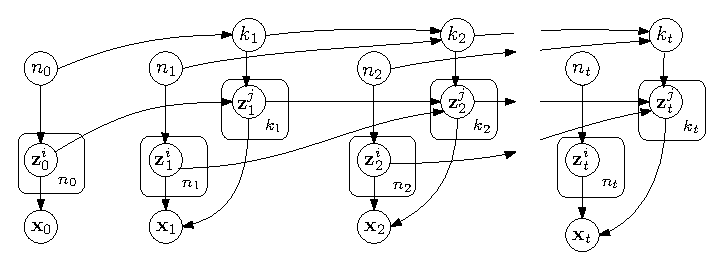
\includegraphics[width=\textwidth]{seq_air}
    \caption{The generative story of sequential AIR.}
    \label{fig:seq_air}
\end{figure}

\begin{figure}
    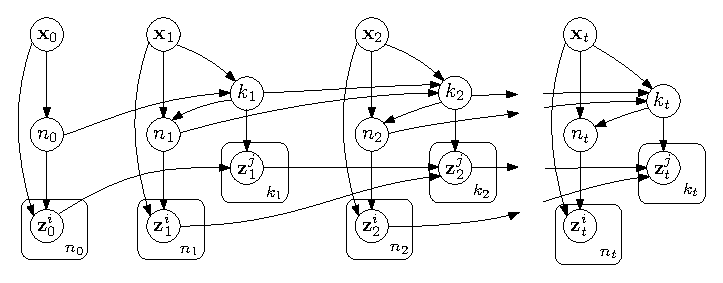
\includegraphics[width=\textwidth]{seq_air_inference}
    \caption{Graphical model for inference in sequential AIR.}
    \label{fig:seq_air_inf}
\end{figure}

\subsection{Sequential Generative Model and Prior}

Let us start by describing the model from the point of view of its generative story. Images are generated by first assuming that, at every time-step, objects are propagated from previous time-step and some new objects can be introduced. Let $k \in \{0, 1, \dots, K\}$,  the number of objects propagated from the previous time-step and let $n \in \{0, 1, \dots, N - k\}$ the number of objects discovered at the current time-step. The maximum of $K \in \mathcal{N}_+$ objects can be propagated and the model can handle up to $N \in \mathcal{N}_+$ total objects, therefore $K \leq N$. Moreover, at every time-step, the model will generate a set of latent variables, one for each object. If we use superscripts $D$ and $P$ to denote latent variables generated by discovery and propagation models, respectively, then the aggregated latent variable $\bzt = \bzt^P \cup \bzt^D$, where $\bzt^P = \{ \bzt^{P, 1}, \dots, \bzt^{P, \kt} \}$ and $\bzt^D = \{ \bzt^{D, 1}, \dots, \bzt^{D, \kt} \}$. Consequently, if we use $m_t = \kt + \nt$ to denote the total number of objects present at time $t$, then $\bzt = \{ \bzt^1, \dots, \bzt^{m_t} \}$. We note that the structure of the latent variables from the discovery and propagation models is the same, and in its simplest form it consists of $\bzt^i = \{ \bzt^{\mathrm{what}, i}, \bzt^{\mathrm{where}, i}, b_t^j \}$. The components represent appearance, location and presence of an object at the given time-step.

 At the first time-step $t = 1$ there are no objects to propagate, so we sample up to $N$ objects from a discovery prior $\p{n_1, \bz_1^D}{N}$. Starting from the second time-step $t=2$, the model first propagates objects by sampling from a propagation prior $\p{k_2, \bz_2^P}{n_1 + k_1, \bz_1}$, where $\bz_1 = \bz_1^D$. The model also samples $n_2$ new objects from the prior $\p{n_2, \bz_2^D}{N - k_2}$. From now on, that is for $t \geq 2$, we set the aggregated latent variable $\bz_t = \{\bz_t^P, \bz_t^D\}$. This process continues up to the final time-step $T$. The images are generated by passing the latent variables $\bzTs$ to the generating model $\p{\bxt}{\bzt}{\theta}$ one at a time. Note that $\bzt$ is a set of up to $N$ latent variables, where each latent variable represents a separate object. The generating model acts separately on every latent variables in the set, and the output random variable of the generating model consists of the sum of outputs of the generative model for each latent variable in the set. \Cref{fig:seq_air} shows the graphical model of the generative story. Please note that the prior for the number of new objects stays the same for every time-step and it is analogous to the prior used by AIR, with the exception that the number of maximum objects can differ.

To make it more formal, we will now give all equations governing the generative process. The prior for the discovery model is defined as follows.
\begin{equation}
\begin{aligned}
    \p{n_t, \bzt^D}{N} &=\\
    \p{n_t}{N} \p{\bzt}{n_t} &= \mathrm{TruncatedGeom} (n_t \mid N) \prod_{i=1}^{n_t} \gauss{\bf{0}, I},
\end{aligned}
\end{equation}
where TruncatedGeom$(n_t \mid N)$ is a geometric distribution, whose support is truncated to $\{0, 1, \dots, N\}$. The propagation model is defined by the following.
\begin{equation}
\begin{aligned}
    \p{k_t, \bzt^P}{m_{t-1}, \bz_{1:t-1}} = \prod_{j=1}^m \p{\bt^{P, j}}{\bz_{1:t-1}^j} \p{\bzt^j}{\bz_{1:t-1}^j} =\\
    \prod_{j=1}^{m_{t-1}} \mathrm{Bernoulli} \left(\bt^{P, j} \mid \psi( \bz_{1:t-1}^j) \right) \gauss{\bzt^j \mid \bm{\mu} (\bz_{1:t-1}^j), \bm{\sigma}^2(\bz_{1:t-1}^j)},
\end{aligned}
\label{eq:prop_prior}
\end{equation}
with $m_t = n_t + k_t$ the total number of objects present at time $t$, $\bz_{1:t-1}^j$ the history of latent variables belonging to object $j$ and $\bz_{1:0}^j = \emptyset$. In the above we reparamterise $k_t$ as a sum of Bernoulli random variables $\bt^{P, j}$, that is $k_t = \sum_{i=1}^m \bt^{P, j}$. Since the probability of propagation $\psi^j$ is different for every object, $k_t$ follows a Poisson-Binomial distribution with $m$ trials. Direct conditioning on the whole history of latent variables is impractical, and therefore we use a learned deterministic RNN $R_\theta^\mathrm{prior}$ to estimate $\psi$, $\mu$ and $\sigma^2$. the RNN shares parameters but maintains a separate hidden state for every object $j$. We can rewrite \Cref{eq:prop_prior} in terms of a simple recurrence as
\begin{equation}
\begin{aligned}
    \p{k_t, \bzt^P}{m_{t-1}, \bz_{1:t-1}} = \p{k_t, \bzt^P}{m_{t-1}, \bm{h}_t^{\mathrm{prior},\ j}} =\\
    \prod_{j=1}^{m_{t-1}} \mathrm{Bernoulli} \left(\bt^{P, j} \mid \psi( \bm{h}_t^{\mathrm{prior},\ j} ) \right) \gauss{\bzt^j \mid \bm{\mu} (\bm{h}_t^{\mathrm{prior},\ j}), \bm{\sigma}^2(\bm{h}_t^{\mathrm{prior},\ j})},
\end{aligned}
\end{equation}
\begin{equation}
    \bm{h}_t^{\mathrm{prior},\ j} = R_\theta^\mathrm{prior} \left( \bz_{t-1}^j, \bm{h}_{t-1}^{\mathrm{prior},\ j} \right).
\end{equation}
Any parameters in the generating model, \eg the parameters of the RNN, can be learnt jointly with the inference model (to be described shortly).
Alternatively, one could use a non-parametric prior for the discrete latent variable $\kTs$, \eg the Indian Buffet Process \citep{Gael2009}. 

Images are created by decoding the latent variables into small `glimpses' that are then transformed to match the size of the original image and summed up. Each latent variable $\bzt^j$ can be decomposed as $\bzt^j = \left\{ \bzt^{j, \mathrm{where}}, \bzt^{j, \mathrm{what}} \right\}$. More formally,
\begin{equation}
    \widehat{\bg}_t^j = f^{\mathrm{dec}}_\theta \left( \bzt^{\mathrm{what}, j} \right),
\end{equation}
\begin{equation}
    \byt^j = f^{\mathrm{STN}} \left( \widehat{\bg}_t^j, \bzt^{\mathrm{where}, j} \right),
\end{equation}
\begin{equation}
    \bm{\mu}_x = \sum_{j=1}^{m_t} \byt^j,
\end{equation}
\begin{equation}
    \widehat{\bx}_t \sim \gauss{ \bxt \mid \bm{\mu}_x, \bm{\sigma}_x^2},
\end{equation}
with the decoder $f^{\mathrm{dec}}$, spatial transformer $f^{\mathrm{STN}}$ and a fixed per-pixel standard deviation $\bm{\sigma}_x^2$.

All components of the generative model taken together specify a joint probability $\p{\bxTs, \bzTs,\nTs,\kTs}{}{\theta}$ over the sequence of images and the corresponding latent variables. We can expand it as
\begin{equation}
\begin{aligned}
    &\p{\bxTs, \bzTs,\nTs,\kTs}{}{\theta} = \prod_{t=1}^T \p{\bxt, \bzt, \nt, \kt}{\bz_{1:t-1}, n_{1:t-1}, k_{1:t-1}}{\theta}\\
%    
    &\qquad= \prod_{t=1}^T \p{\bxt}{\bzt}{\theta} \p{\bzt, \nt, \kt}{\bz_{1:t-1}, n_{1:t-1}, k_{1:t-1}}{\theta}\\
%    
    &\qquad= \prod_{t=1}^T \underbrace{\p{\bxt}{\bzt}{\theta}}_\mathrm{generation} \quad \underbrace{\p{\bzt^D, \nt}{\bzt^P, \kt}{\theta}}_\mathrm{discovery} \quad \underbrace{\p{\bzt^P, \kt}{\bz_{1:t-1}, n_{1:t-1}, k_{1:t-1}}{\theta}}_\mathrm{propagation}.
\end{aligned}
\end{equation}
In the second line we used the fact that the observation at time $t$ is conditionally independent of latent variables at previous time-steps given the current ones. In the third line we decomposed $\bzt$ as the union of latent variables corresponding to the discovered objects $\bzt^D$ and propagated objects $\bzt^P$. Only the latter depend on the history of latent variables; the former depend only on what is captured in propagation to the current step. The last term can be decomposed as
\begin{equation}
\begin{aligned}
&\p{\bzt^P, \kt}{\bz_{1:t-1}, n_{1:t-1}, k_{1:t-1}}{\theta}\\
%
&\qquad= \int \p{\bzt^P, \kt}{\bz_{t-1}, n_{t-1} + k_{t-1}, \bm{h}_t^P}{\theta} \p{\bm{h}_t^P}{\bm{h}_{t-1}^P, \bz_{t-1}}{\theta} \dint \bm{h}_t^\mathrm{prior}\\
%
&\qquad= \p{\bzt^P, \kt}{\bz_{t-1}, m_{t-1}, \bm{h}_t^\mathrm{prior}}{\theta} \lvert_{\bm{h}_t^\mathrm{prior} = R^\mathrm{prior}_\theta \left( \bm{h}_{t-1}^\mathrm{prior}, \bz_{t-1} \right)},
\end{aligned}
\end{equation}
where we introduce the hidden state $\bm{h}_t^P$ of the RNN used for propagating objects through time. Computation of the state is deterministic and therefore $\p{\bm{h}_t^\mathrm{prior}}{\bm{h}_{t-1}^\mathrm{prior}, \bz_{t-1}}{\theta}$ is a Dirac distribution centred on $\bm{h}_t^P$, which further simplifies computation. In the second line we also used the fact that object propagation depends only on the number of objects present at the previous time-step and it does not matter whether the objects were propagated from previous time-step or newly discovered.

\subsection{Inference}
To infer the latent variables, we have to invert the generative model. To do so, the inference model has to take into account the observations $\bxTs$ and produce sequences of sets of latent variables $\bzTs$. Similar to the generative process, inference uses a two-step approach, whereby it propagates objects from previous time-steps and then tries to discover new objects. Let us start by defining the approximate posterior distribution over all latent variables.
\begin{equation}
\begin{aligned}
    &\q{\bzTs, \nTs, \kTs}{\bxTs}{\phi} \\
%    
    &\qquad= \prod_{t=1}^T  \q{\bzt, \nt, \kt}{\textcolor{red}{\bxts}, \bz_{1:t-1}, n_{1:t-1}, k_{1:t-1}}{\phi}\\
%    
    &\qquad= \prod_{t=1}^T  \q{\bzt, \nt, \kt}{\textcolor{red}{\bxt}, \textcolor{blue}{\bz_{1:t-1}, n_{1:t-1}, k_{1:t-1}}}{\phi}\\
%    
    &\qquad= \prod_{t=1}^T  \q{\bzt, \nt, \kt}{\bxt, \textcolor{blue}{\bz_{t-1}, n_{t-1}, k_{t-1}}, \bm{h}_t^q}{\phi}\lvert_{\bm{h}_t^q = R^q_\phi \left( \bz_{t-1}, \bm{h}_{t-1}^q \right)} \\
%    
    &\qquad= \prod_{t=1}^T  \qd{\bzt^D, \nt}{\bxt, \bzt^P, \kt}{\phi} \qp{\bzt^P, \kt}{\bxt, \bz_{t-1}, \textcolor{red}{k_{t-1} + n_{t-1}}, \bm{h}_t^q}{\phi} \\
%    
    &\qquad= \prod_{t=1}^T  \underbrace{ \qd{\bzt^D, \nt}{\bxt, \bzt^P, \kt}{\phi}}_\mathrm{discovery} \quad \underbrace{\qp{\bzt^P, \kt}{\bxt, \bz_{t-1}, \textcolor{red}{m_{t-1}}, \bm{h}_t^q}{\phi}}_\mathrm{propagation} 
\end{aligned}
\end{equation}
In the second line we use the product rule to rewrite the joint distribution as a temporal chain. In the third line we introduce the assumption that latent variables are conditionally independent of the past observations given the corresponding latent variables. In the fourth line we substituted the dependency on the history of latent variables by introducing a Markovian hidden state $\bm{h}_t^q$. We assume that the hidden state follows a Dirac distribution and therefore the associated integral collapses to a single value. In line five we decompose the latent variable $\bzt$ into the ones introduced by the discovery and propagation steps, respectively. We also omit the value of the hidden state to reduce clutter. In line six we explicitly condition the propagation step on the number of latent variables in the previous time-step.

We start by describing the propagation model $\q{}{}{\phi}$. We would like to condition propagation of objects on other propagated objects at the current time-step, and therefore we decompose inference into a sequence of steps.
\begin{equation}
\begin{aligned}
    &\qp{\bzt^P, \kt}{\bxt, \bz_{t-1}, m_{t-1}, \bm{h}_t^q}{\phi}\\
%    
    &\qquad= \prod_{i=1}^{m_{t-1}} \qp{\bzt^{P, i}, \bt^{P, i}}{\bxt, \bz_{t-1}^i, \bm{h}_t^q, \textcolor{red}{\bzt^{P, 1:i-1}}}{\phi}\\
%    
    &\qquad= \prod_{i=1}^{m_{t-1}} \qp{\bzt^{P, i}, \bt^{P, i}}{\bxt, \bz_{t-1}^i, \bm{h}_t^q, \textcolor{blue}{\bm{h}_t^{P, i}}}{\phi} \lvert_{\bm{h}_t^{P, i} = R_\phi^P \left(  \bzt^{P, i-1}, \bt^{P, i-1} \bm{h}_t^{P, i-1} \right)}
\end{aligned}
\end{equation}
$\bzt^{P, 0}$ and $bt^{P, 0}$ start as zeros and  $\bm{h}_t^{P, 0}$ is randomly initialised and learnable. It is worth noting that $m_t = \sum_{i=1}^{m_{t-1}} \bt^{P,i} \leq m_{t-1}$, therefore propagation can forget objects, but it cannot introduce any new ones. At the end of the propagation stage, the hidden state $\bm{h}_t^{S, \kt}$ should contain information about all the propagated objects and can be used to condition the discovery stage.

To handle object discovery, we follow the implementation of AIR, with the difference that we condition on the hidden state of the propagation phase $\bm{h}_t^{P, \kt}$ and that there is a variable maximum number of steps. It defines a sequential inference procedure, where the model attends to and explains different regions of the image, one at a time. The approximate posterior distribution is defined by \Cref{eq:air_posterior,eq:air_recurrence,eq:air_factorisation}.
We redefine it here to account for temporal dependencies and conditioning. The approximate posterior distribution for discovered objects is given by
\begin{equation}
\begin{aligned}
    &\qd{\bzt^D, \nt}{\bxt, \textcolor{red}{\bzt^P}, \kt}{\phi}\\
%    
    &= \qd{\bzt^D, \nt}{\bxt, \textcolor{red}{\bm{h}_t^{P, \kt}}, \kt}{\phi}\\
%    
    &= \qd{\bt^{D, \nt + 1} = 0}{\bxt, \textcolor{blue}{\bzt^{D, 1:\nt}}, \bm{h}_t^{P, \kt}, \kt}{\phi} \prod_{i=1}^{\nt} \qd{\bt^{D, i}, \bzt^{D, i}}{\bxt, \textcolor{blue}{\bzt^{D,1:i-1}}, \bm{h}_t^{P, \kt}, \kt}{\phi}\\
%    
    &= \qd{\bt^{D, \nt + 1} = 0}{\bxt, \textcolor{blue}{\bm{h}_t^{D, \nt}}, \bm{h}_t^{P, \kt}, \kt}{\phi} \prod_{i=1}^{\nt} \qd{\bt^{P, i}, \bzt^{D, i}}{\bxt, \textcolor{blue}{\bm{h}_t^{D, i-1}}, \bm{h}_t^{P, \kt}, \kt}{\phi},\\
%    
%    &\text{where}\\
%    
\end{aligned}
\end{equation}
where
\begin{equation}
\begin{aligned}
    &\qquad \bm{h}_t^{D, i} = R_\phi^D \left( \bzt^{D, i}, \bm{h}_t^{D, i-1} \right),\\
%    
    &\qquad \qd{\bt^{D, i}}{\bxt, \bzt^{D, 1:i}, \bm{h}_t^{P, \kt}, \textcolor{red}{\kt}}{\phi} = 
    \begin{cases}
        \qd{\bt^{D, i}}{\bxt, \bzt^{D, 1:i}, \bm{h}_t^{P, \kt}}, & \text{if}\ i \leq N-\kt \\
        0, & \text{otherwise}
    \end{cases},\\
%    
    &\qquad \qd{\bt^{D, i} \textcolor{blue}{= 0}}{\bxt, \bzt^{D, 1:i}, \bm{h}_t^{P, \kt}, \kt}{\phi} 
    = 1 - \qd{\bt^{D, i}}{\bxt, \bzt^{D, 1:i}, \bm{h}_t^{P, \kt}, \kt}{\phi}.
\end{aligned}
\end{equation}

\subsection{Variational Lower Bound}
Given the specification of the prior distribution and the inference model, we can derive the evidence lower bound (ELBO).
\begin{equation}
\begin{aligned}
    &\loss[APDR]{\phi, \theta} = \expc{ \log \frac{ \p{\bzTs, \nTs, \kTs, \bxTs}{}{\theta} }{ \q{\bzTs, \nts, \kts}{\bxTs}{\phi} } }{}{ \q{}{}{\phi} }\\
    %
    &= \expc{ \log \p{\bxTs}{\bzTs}{\theta} }{}{ \q{}{}{\phi} } \\
%    
    &\qquad \qquad - \kl{\q{\bzTs, \nTs, \kTs}{\bxTs}{\phi}}{\p{\bzTs, \nTs, \kTs}{}{\theta}}.
\end{aligned}
\end{equation}
The KL divergence term cannot be computed analytically due to non-linear temporal dependencies, and we have to resort to a Monte-Carlo approximation. The latter can be rewritten as a sum of per time-step components. 
%\begin{equation}
%\begin{aligned}
%    &\kl{\q{\bzTs, \nTs, \kTs}{\bxTs}{\phi}}{\p{\bzTs, \nTs, \kTs}{}{\theta}}\\
%%    
%    &= \dots\\
%%    
%    &\approx \sum_{t=1}^T \operatorname{KL}_t(\cdot)
%\end{aligned}
%\end{equation}
Let $\bm{\beta} = \{ \bz, n, k, \bm{h} \}$ denote all latent variables and all hidden states. We have that 
\todo{Make sure the below is correct!}
\begin{equation}
\begin{aligned}
    &\kl{\q{\bzTs, \nTs, \kTs}{\bxTs}{\phi}}{\p{\bzTs, \nTs, \kTs}{}{\theta}}\\
    %    
    &= \kl{\q{\bm{\beta}_{1:T}}{\bxTs}{\phi}}{\p{\bm{\beta}_{1:T}}{}{\theta}}\\
%    
    &= \int \q{\bm{\beta}_{1:T}}{\bxTs}{\phi} \log{\frac{\q{\bm{\beta}_{1:T}}{\bxTs}{\phi}}{\p{\bm{\beta}_{1:T}}{}{\theta}}} \dint \bm{\beta}_{1:T}\\
%    
    &= \int \prod_{t=1}^T \left[ \q{\bm{\beta}_t}{\textcolor{red}{\bxts, \bm{\beta}_{1:t-1}}}{\phi} \log{\frac{\q{\bm{\beta}_{1:T}}{\bxTs}{\phi}}{\p{\bm{\beta}_{1:T}}{}{\theta}}} \right] \dint \bm{\beta}_{1:T} \\
%    
    &= \int \prod_{t=1}^T \left[ \q{\bm{\beta}_t}{\textcolor{red}{\bxt, \bm{\beta}_{t-1}}}{\phi} \log{\frac{\q{\bm{\beta}_{1:T}}{\bxTs}{\phi}}{\p{\bm{\beta}_{1:T}}{}{\theta}}} \right] \dint \bm{\beta}_{1:T}\\
%    
    &= \int \prod_{t=1}^T \q{\bm{\beta}_t}{\bxt, \bm{\beta}_{t-1}}{\phi} \left[ \sum_{t=1}^{\textcolor{blue}{T}} \log{\frac{ \q{\bm{\beta}_t}{\bxt, \bm{\beta}_{t-1}}{\phi} }{ \p{\bm{\beta}_t}{\bm{\beta}_{t-1} }{\theta}}} \right] \dint \bm{\beta}_{1:T}\\
%    
    &= \textcolor{red}{\int \prod_{t=1}^T} \q{\bm{\beta}_t}{\bxt, \bm{\beta}_{t-1}}{\phi} \left[ \sum_{t=1}^{\textcolor{blue}{t}} \log{\frac{ \q{\bm{\beta}_t}{\bxt, \bm{\beta}_{t-1}}{\phi} }{ \p{\bm{\beta}_t}{\bm{\beta}_{t-1} }{\theta}}} \right] \textcolor{red}{\dint \bm{\beta}_{1:T}}\\
%    
    &= \textcolor{red}{\prod_{t=1}^T \int} \underbrace{ \q{\bm{\beta}_t}{\bxt, \bm{\beta}_{t-1}}{\phi} }_{\textcolor{blue}{\text{is that ok?}}} \left[ \sum_{t=1}^t \log{\frac{ \q{\bm{\beta}_t}{\bxt, \bm{\beta}_{t-1}}{\phi} }{ \p{\bm{\beta}_t}{\bm{\beta}_{t-1} }{\theta}}} \right] \textcolor{red}{\dint \bm{\beta}_{t-1:t} }\\
%    
    &\approx \sum_{t=1}^T \operatorname{KL}_t(\cdot)
\end{aligned}
\end{equation}

where
\begin{equation}
\begin{aligned}
    \operatorname{KL}_t(\cdot) = &\frac{1}{L} \sum_{i=l}^L \log{\frac{ \q{\bzt^{(l)}, \nt^{(l)}, \kt^{(l)}}{\bxt, \bz_{t-1}^{(l)}, n_{t-1}^{(l)}, k_{t-1}^{(l)}, \bm{h}_t^{q,\ (l)}}{\phi} }{ \p{\bxt, \bzt^{(l)}, \nt^{(l)}, \kt^{(l)}}{\bz_{1:t-1}^{(l)}, n_{1:t-1}^{(l)}, k_{1:t-1}^{(l)}}{\theta} }},\\
%    
    \text{with}\\
%    
    &\bzTs^{(l)}, \nTs^{(l)}, \kTs^{(l)} \sim \q{\bzTs, \nTs, \kTs}{\bxTs}{\phi},\\
%    
    &\bm{h}_t^{q,\ (l)} = R^q_\phi \left( \bz_{t-1}{(l)}, \bm{h}_{t-1}^{q,\ (l)} \right)
\end{aligned}
\end{equation}
The above approximation allows us to rewrite the ELBO as a sum of per time-step components, namely
\begin{equation}
    \loss[APDR]{\phi, \theta} \approx \sum_{t=1}^T \expc{ \log \p{\bxt}{\bzt}{\theta} }{}{ \q{}{}{\phi} } - \operatorname{KL}_t(\cdot),
\end{equation}
which can be useful if we wanted to use a particle filter estimator of the ELBO, \emph{cf.} \Cref{sec:fivo}.